\documentclass[letterpaper,12pt,addpoints]{exam}
\usepackage[utf8]{inputenc}
\usepackage[english]{babel}

\usepackage[top=1in, bottom=1in, left=0.75in, right=0.75in]{geometry}
\usepackage{amsmath,amssymb}

\usepackage{enumitem}
\usepackage{hyperref}

\usepackage[english]{babel}
\usepackage{amssymb}
\usepackage{amsmath}
\usepackage{amsfonts}
\usepackage{epsfig, graphics}
\usepackage{latexsym}
\usepackage[parfill]{parskip}
\usepackage{url}
\usepackage{titlesec}
% \usepackage{mysymbols}
\usepackage{tikz}
\usepackage{fancyvrb} % for "\Verb" macro

% ~ additional packages ~
\usepackage{booktabs} % fancy tables
\usepackage{caption} % captionof
\usepackage{comment}
%\usepackage{listings} % python code
\usepackage{xcolor}
\usepackage{listings}
%\usepackage{exsheets}


\newcommand{\university}{Georgia Institute of Technology}
\newcommand{\faculty}{Faculty of Interactive Computing}
\newcommand{\class}{CS8003}
\newcommand{\examnum}{ASSIGNMENT \#1}
\newcommand{\content}{Deep Reinforcement Learning}
\newcommand{\examdate}{2024/10/22}

\pagestyle{headandfoot}
\firstpageheader{}{}{}
\firstpagefooter{}{Page \thepage\ of \numpages}{}
\runningheader{\class}{\examnum}{\examdate}
\runningheadrule
\runningfooter{}{Page \thepage\ of \numpages}{}

\begin{document}

\title{\Large \textbf{\university\\ \faculty\\
\bigskip
\class -- \examnum \\ \content}}
\author{Instructor: Prof. Animesh Garg}
\date{Due date: \examdate}

\maketitle
\begin{flushleft}
\makebox[12cm]{\textbf{Name}:\ \hrulefill}
\medskip
\makebox[12cm]{\textbf{Student Number}:\ \hrulefill}
\end{flushleft}
\noindent \rule{\textwidth}{1pt}

\noindent This writing assignment contains \numpages\ pages (including this cover page) and \numquestions\ questions. Total of points is \numpoints.\\
Good luck and Happy reading work!

\vspace{15pt}

The assignment must be completed before \textbf{11:59am on Tuesday, Oct 22, 2024}. Upload your submission as one ZIP file on Canvas. 

This assignment consists of two parts: a writing question and a coding question. For the writing question, your submission should be typeset, and all answers must be clearly legible. You are required to submit a PDF file containing your responses to the writing question (you may directly type your answer here and submit the file). For the coding question, you need to submit your code along with the running results, including the reward plot and a testing GIF file. Clearly specify which algorithm you are using to generate these plots. The coding question is divided into two sections: the fundamental coding questions (\texttt{hw1\_basic.ipynb}) and the advanced coding questions (\texttt{hw1\_advanced.ipynb}). In general, it is recommended that you complete the writing questions first, followed by the basic coding questions, and finally the advanced coding questions. Note that prior knowledge may be required to complete the advanced section. \textbf{\textcolor{blue}{Please ensure that you start this assignment as early as possible, as it will take time to run and fine-tune your code.}}



The assignment must be completed by each student alone. Collaboration with other students is strictly prohibited. 
\textbf{
Questions may be asked on Ed in case of unclear formulations. Do not post answers, partial answers or hints to answers!} Furthermore, we expect all students to adhere to the standards of academic integrity of the Georgia Institute of Technology. 



\clearpage
\section{Reinforcement Learning Fundamentals (10 points)}

\begin{questions}
    \question[3]{
        Describe the difference between \textit{supervised learning} and \textit{reinforcement learning}. Use two application examples to highlight the difference.
    }
    \question[4]{
        Describe how one of your examples from the first question can be formalized with a MDP. State all formal parts of the MDP and sketch how the formal structure relates to your problem.
    }
    \question[3]{
        When dealing with \textit{infinite horizon problems}, it is common to include a \textit{discount factor}. Describe, in your own words, the role the discount factor plays in the reinforcement learning problem and what problem might occur if the discount factor is set to 1, and what problem might occur if the discount factor is set to 0.
    }
\end{questions}
\newpage

\section{Multiple Choices Questions (16 points)}
For each of the following multiple-choice questions, select the correct answer(s). There may be more than one correct option per question. To simplify grading, the multiple-choice section will be uploaded to Canvas. \textbf{\textcolor{blue}{Complete this part on Canvas, as answers not submitted there will not be graded! We will open this section on Canvas as soon as possible!}}


\begin{questions}
\question[2] Suppose we are having a well-defined finite grid world MDP problem with terminal state included. For each state, you will have your reward $R$ defined properly and $R\ge 0$ for every grid. Suppose that we want to re-design the reward function there. For which of the following new reward functions would \textbf{guarantee} the optimal policy \textbf{remain unchanged}? Let $R(s,a,s')$ be the original reward function. 

\begin{checkboxes}
 \choice $R_1(s,a,s') = 10R(s,a,s')$
 \choice $R_2(s,a,s') = 1+R(s,a,s')$
 \choice $R_3(s,a,s') = R(s,a,s')^2$
 \choice $R_4(s,a,s') = 1$
 \choice None
\end{checkboxes}

\question[2] In TD learning with linear VFA (value function approximation), which of the following statement is true? 
\begin{checkboxes}
\choice To present a value function with a weighted linear combination of features, we can write $V(s; w) = x(s)^Tw(s)$
\choice For SARSA using VFA,  
$\Delta w = \alpha(r+\gamma \hat{Q(s', a'; w)} - \hat{Q(s, a; w)})\nabla_w\hat{Q(s', a'; w)}$
\choice Consider we are using non-linear value function approximation, then during the weights update, we just need to re-calculate $\nabla_w\hat{Q(s, a; w)}$. 
\choice None of the above
\end{checkboxes}


\question[2] Which statement is true about Policy gradient?
\begin{checkboxes}
 \choice Policy gradient can be computed with automatic differentiation when policy is a neural network. True
 \choice Policy gradient is on-policy. True
 \choice Policy gradient can also derive off-policy variants using importance sampling. True
 \choice In Vanilla policy gradient, the condition number is small when computing the gradient. False
 \choice In covariant/natual policy gradient, we re-scale the gradient properly to improve the optimization. True
\end{checkboxes}

\question[2] Which statement is true about Policy gradient? (Hint: two options are correct.)
\begin{checkboxes}
 \choice Policy gradient will have a low variance since gradient is unbiased. 
 \choice Policy gradient will have a high variance since huge amounts of rollouts will introduce noisy gradients.
 \choice Using a larger batch in Policy gradient will lead to high variance.
 \choice Tweaking the learning rate such as using adaptive step size rules can reduce the variance in Policy gradient.
 \choice Having a fixed learning rate can reduce the variance in Policy gradient.
\end{checkboxes}

\question[2] Which statement is true about Policy gradient?
\begin{checkboxes}
\choice In Policy gradient, we subtract the baseline to reduce the variance. True
\choice In Policy gradient, subtracting the baseline may introduce bias. False
\choice In policy gradient, The baseline is essentially a proxy for the expected actual return. True
\choice None of the above
\end{checkboxes}

\question[2] Which statement is true about Actor-critic?
\begin{checkboxes}
 \choice Actor-Critic is a Temporal Difference(TD) version of Policy gradient.
 \choice Both actor and critic are improving overtime.
 \choice Consider actor-critic with discount, we prefer to discount the whole gradient because we care about the whole trajectory. False
 \choice We usually design actor and critic with shared features when states are high dimensional such as image state representation. True
 \choice In online actor-critic, we have both synchronized and asynchronous version.
\end{checkboxes}


\question[2] What statements are true about \textbf{on-policy} algorithms?
\begin{checkboxes}
 \choice They are able to reuse data from different policies in the past directly
 \choice They are \textbf{not} able to reuse data from different policies in the past directly
 \choice They are always more sample efficient than off-policy algorithms
 \choice They cannot be used in discrete state-action spaces
 \choice None of the above
\end{checkboxes}
\question[2] Why do we need the log ratio trick in REINFORCE?
\begin{checkboxes}
\choice Because we cannot differentiate the gradient estimator otherwise
\choice Because the original authors did not not like automatic differentiation
\choice Because the gradient estimate has too much stochasticity
\choice Because it helps with exploration 
\choice None of the above
\end{checkboxes}
\end{questions}

\clearpage


\section{Calculation Questions on Tabular Q-Leaning(8 points)}

\begin{questions}
\question[4] Consider a system with two states and two actions. You perform actions and observe the
rewards and transitions listed below. Each step lists the current state, reward, action and resulting transition as $S_i;R=r;a_k:S_i \rightarrow S_j$. Perform Q-learning using a learning rate $\alpha=0.5$ and discount factor of $\gamma$ = 0.5 for each step. The $Q$ entries are initialized to zero. After step 3, what is $Q(S_2, a_1)$?

Step 1: $S_1;R=-10;a_1:S_1 \rightarrow S_1$ \\
Step 2: $S_1;R=-10;a_2:S_1 \rightarrow S_2$ \\
Step 3: $S_2;R=+20;a_1:S_2 \rightarrow S_1$

\begin{solution}[2in]
\end{solution}

\question[4] In the same setup as the previous question, what if you are performing SARSA algorithm and you are having an extra step 4 as followed. What is $Q(S_2, a_1)$ after performing the 4 steps? 

Consider a system with two states and two actions. You perform actions and observe the
rewards and transitions listed below. Each step lists the current state, reward, action and resulting transition as $S_i;R=r;a_k:S_i \rightarrow S_j$. Perform SARSA using a learning rate $\alpha=0.5$ and discount factor of $\gamma=1$ for each step. The $Q$ entries are initialized to zero.


Step 1: $S_1;R=-10;a_1:S_1 \rightarrow S_1$ \\
Step 2: $S_1;R=-10;a_2:S_1 \rightarrow S_2$ \\
Step 3: $S_2;R=+20;a_1:S_2 \rightarrow S_1$ \\
Step 4: $S_1;R=+10;a_1:S_1 \rightarrow S_2$


\end{questions}

\newpage

\section{Analyzing a Modern Algorithm: DDPG (14 points)}
In this section, we will work our way towards the formulation of a modern high performance reinforcement learning algorithm. As we shall see, this algorithm is ultimately derived from similar principles as the reinforcement learning algorithms discussed in class, with adjustments to increase its stability and efficiency.
In particular, we will discuss the Deep Deterministic Policy Gradient (DDPG) algorithm. The DDPG algorithm can be found in a simplified form in Figure \ref{fig:ddpg}.

\begin{figure}[h!]
    \centering
    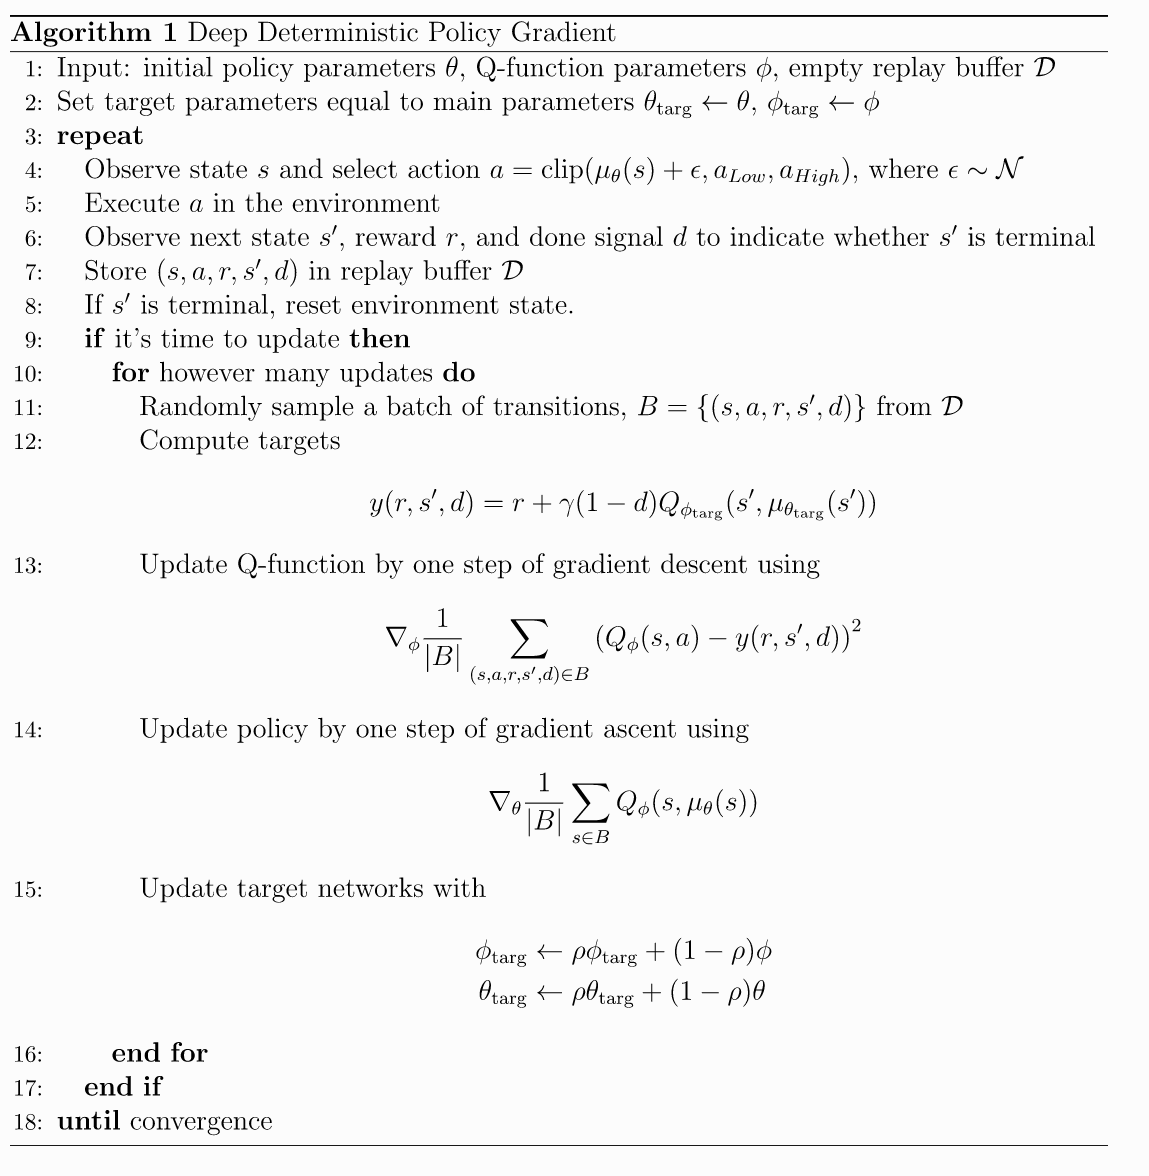
\includegraphics[width=0.95\textwidth]{imgs/ddpg.png}
    \caption{DDPG Algorithm}
    \label{fig:ddpg}
\end{figure}


\newpage 

\begin{questions}
    \question[3]{
    State a similarity/relationship of this algorithm to \textbf{2 different algorithms} that were discussed in class, \textbf{one similarity per algorithm}.
    
    \begin{solution}[2.5in]
    \end{solution}
    }

    \question[4]{
    DDPG aims to learn a Q-function within a continuous action space. Of course, we learned in class that this is generally quite difficult. \\
    (i) (1 point) Please state the reason that this is so.\\
    (ii) (3 points) Subsequently, state and explain the approach adopted by DDPG to avoid the issue you raised, with reference to the algorithm written above.
    \begin{solution}[3in]
    \end{solution}
    }
    
    \newpage
    \question[5]{
    State and explain one alternate approach to solve the issue raised in the previous part of this question, using pseudo-code to illustrate your idea. What is one benefit and one drawback of this approach compared to DDPG?
    
    \begin{solution}[4.5in]
    \end{solution}
    }
    
    \question[2]{
    The policy portion of the update is not the same as the standard policy gradient, and instead makes an assumption on some property of the $Q$ function.
    
    State the assumption on $Q$ that DDPG is using here for their policy update, and explain how it justifies the expression in gradient ascent.
    
    \begin{solution}[2in]
    \end{solution}
    }
    
    \newpage
    
    
\end{questions}

\newpage

\section{Reinforcement Learning Application (18 points)}
Reinforcement learning method can be widely used in many different field. For this question, we will explore deep reinforcement learning methods in traffic signal control (TSC) applications. 
Consider a simple TSC problem. In a single four-way intersection, each direction is controlled with green, red and yellow phases by a traffic light. The main goal of TSC is providing safe, effective and reliable transportation systems to participants. 
\begin{questions}
    \question[2]{
        Please briefly state that why TSC problem can be described as MDP. 
        \begin{solution}[2in]
        \end{solution}
    }
    \question[4]{
        Dealing with the TSC problem on simulators by using RL algorithms requires a good problem formulation in several parts: state, action, reward definitions and neural network structure. In this single four-way intersection situation, please describe what is your state and action in this problem and give a concrete example of each. You need to describe your state and action clearly on what each feature in your state and action represent of and how you are extracting this information. 
    }
    \begin{solution}[3in]
        \end{solution}
    
    \newpage
    \question[4]{
        The role of reward in RL is analyzing the quality of taken action with respect to the state. Please list at least 2 possible scenarios that might happen in this TSC problem and write the mathematical representation (such as $r_0 = \sum_i A_i^2 $ where A is ...) to describe how you are going to penalize or award the agent for this scenario. 
    }
    \begin{solution}[3in]
        \end{solution}
        
    \question[3]{
        Noticing that a car accident must be prevented in TSC. We add a safety constraint $\mathcal C=\{c:S\rightarrow \{0,1\}\}$ that the agent must satisfy. With this extra constraint, we call it constrained MDP (CMPD). One could also argue that we can add a penalty to the agent when car accident happens. Please clarify what is the difference between C-MDP and adding reward penalty.
    }
    \begin{solution}[2in]
        \end{solution}
    
    \newpage
    \question[3]{
    Supposed that we are using Policy Optimization method to solve the CMDP problem describing above. What could be a problem compared to MDP? 
    }
    \begin{solution}[2.5in]
        \end{solution}
    
    
    \question[2]{
    Please briefly describe one intuition to solve the problem in the previous question. 
    }
    \begin{solution}[0.5cm]
        \end{solution}

 
\end{questions}


\newpage

\section{Coding Questions (65 points)}
This section provides instructions for the coding assignment. The coding questions are divided into two parts: basic coding questions (covering algorithms taught in class) and advanced coding questions (implementing a commonly used model-free algorithm, not covered in class but guided step-by-step). Please clone the repository from \url{https://github.com/pairlab/cs8803drl-fall24.git} to access the code. Follow the instructions provided to complete the coding assignment step by step.

\textbf{Before beginning the coding tasks, follow the instructions in the \texttt{README.md} file to set up a Python environment for running the code. You may use either a GPU or CPU to train your algorithm.
}


\textbf{\textcolor{blue}{Notice:}} \textbf{\textcolor{blue}{All hyperparameters inside the \texttt{Hyper-parameters Tuning} cell may require adjustment. Please allocate sufficient time to complete the coding questions.}}


\textbf{You are free to add any additional functions or methods to the code if you find that simply completing the TODO sections is not sufficient to make the code run properly.}

\subsection{Basic Coding Questions (40 points)}
For the basic coding question, the code is provided in \texttt{hw1\_basic.ipynb}. Ensure that you run all cells in this notebook and save the reward plot and GIF file as \texttt{\{algo\_name\}\_returns.png} and \texttt{\{algo\_name\}\_policy.gif}, respectively. Follow the instructions for each algorithm to complete the corresponding functions in the \texttt{/src} directory. 

If you run the code cells in \texttt{hw1\_basic.ipynb}, \texttt{\{algo\_name\}\_returns.png} and \texttt{\{algo\_name\}\_policy.gif} will be automatically generated under the \texttt{artifacts/} folder. In the basic coding task, we are using the "LunarLander-v2" environment with discrete action space. You are encouraged to try different discrete or continuous action environments in Gym. You can also explore more complex tasks from Gym-Atari or MuJoCo (note that these may require additional package installations).


\begin{questions}


\question[10]{
\textbf{REINFORCE algorithm: } \\
Completing the code in \texttt{src/network.py} and \texttt{src/reinforce.py} based on the TODO instructions should be sufficient to run the REINFORCE algorithm. You can tune the parameters inside the \texttt{Hyper-parameters Tuning} cell in the \texttt{hw1\_basic.ipynb} file if you find that the provided values are not sufficient to achieve the desired results.
}

\question[10]{
\textbf{Simple Q-iteration (no experience replay + target network): } \\
Completing the code in \texttt{src/network.py} and \texttt{src/q\_iter.py} based on the TODO instructions should be sufficient to run the Q-iteration algorithm. You can tune the parameters inside the \texttt{Hyper-parameters Tuning} cell in the \texttt{hw1\_basic.ipynb} file if you find that the provided values are not sufficient to achieve the desired results.
}


\question[10]{
\textbf{DQN (Deep Q-learning + experience replay + target network): } \\ 
Completing the code in \texttt{src/network.py} and \texttt{src/dqn.py} based on the TODO instructions should be sufficient to run the DQN algorithm. You can tune the parameters inside the \texttt{Hyper-parameters Tuning} cell in the \texttt{hw1\_basic.ipynb} file if you find that the provided values are not sufficient to achieve the desired results.
}

\question[10]{
\textbf{Actor-Critic: }\\ 
Completing the code in \texttt{src/network.py} and \texttt{src/ac.py} based on the TODO instructions should be sufficient to run the Actor-Critic algorithm. You can tune the parameters inside the \texttt{Hyper-parameters Tuning} cell in the \texttt{hw1\_basic.ipynb} file if you find that the provided values are not sufficient to achieve the desired results.
}
\end{questions}

\subsection{Advanced Coding Questions (25 points)}
For the advanced coding question, the code is provided in \texttt{hw1\_advanced.ipynb}. Ensure that you complete and run all cells in this notebook and save the reward plot \texttt{sac\_returns.png}.

In the advanced coding task, we are using the "Pendulum-v1" environment with continuous action space. You are encouraged to try different continuous action environments in Gym. You can also explore more complex tasks from Gym-Atari or MuJoCo (note that these may require additional package installations).

\begin{questions}
\question[25]{
\textbf{Soft Actor-Critic: }\\ 
Complete the code in \texttt{hw1\_advanced.ipynb} based on the TODO instructions. You can tune the parameters inside the \texttt{Hyper-parameters Tuning} cell in the \texttt{hw1\_advanced.ipynb} file if you find that the provided values are not sufficient to achieve the desired results.
}
\end{questions}

\newpage
\section*{Checkbox for Assignment Submission}

\textbf{Congratulations on completing Assignment 1! We have created a checklist for you to double-check your submission. The files you need to submit are:}

\begin{itemize}[left=0pt, label={\textcolor{blue}{$\square$}}]
    \item \textbf{hw1.zip}: a zip file with your completed PDF and code.
    \begin{itemize}[left=20pt, label={\textcolor{blue}{$\square$}}]
        \item \textbf{Python files}:\\ \texttt{ac.py}, \texttt{dqn.py}, \texttt{networks.py}, \texttt{q\_iter.py}, \texttt{reinforce.py}
        \item \textbf{Jupyter Notebook files}:\\ \texttt{hw1\_basic.ipynb}, \texttt{hw1\_advanced.ipynb}
        \item \textbf{Coding results}:\\ \texttt{ac\_policy.gif}, \texttt{ac\_returns.png},\\ \texttt{dqn\_policy.gif}, \texttt{dqn\_returns.png},\\ \texttt{q\_iteration\_policy.gif}, \texttt{q\_iteration\_returns.png},\\ \texttt{reinforce\_policy.gif}, \texttt{reinforce\_returns.png},\\ \texttt{sac\_returns.png}, \texttt{sac\_policy.gif} (optional)
    \end{itemize}
    \item \textbf{Writing assignment PDF file}: \texttt{CS8803\_DRL\_A1.pdf}
    \item \textbf{hw1\_basic.pdf}: \\ Convert the \texttt{hw1\_basic.ipynb} to a PDF file \textbf{\textcolor{blue}{containing your running results.}}
    \item \textbf{hw1\_advanced.pdf}:\\  Convert the \texttt{hw1\_advanced.ipynb} to a PDF file \textbf{\textcolor{blue}{containing your running results.}}
    \item \textbf{Completing the Multiple Choices Questions on Canvas.}
\end{itemize}




\end{document}
